%% ============================================================
%% RFP_Final_Report.tex
%% Real-time/Field-Based Research Project Report
%% CVR College of Engineering — Department of CSE
%% ============================================================

% ---- R2: Document class and packages -----------------------
\documentclass[12pt,a4paper]{report}
\usepackage[utf8]{inputenc}
\usepackage{mathptmx}           % Times New Roman equivalent
\usepackage{setspace}           % Line spacing
\onehalfspacing                 % 1.5 line spacing
\usepackage[
  left=3.75cm,
  right=2.5cm,
  top=2.5cm,
  bottom=2.5cm
]{geometry}                     % Margins as per template
\usepackage{fancyhdr}           % Page numbers at bottom center
\usepackage{graphicx}           % For college logo image
\usepackage{hyperref}           % For clickable TOC
\usepackage{titlesec}           % Section title formatting
\usepackage{booktabs}           % Professional tables
\usepackage{longtable}          % Multi-page tables
\usepackage{array}              % Enhanced column formatting
\usepackage{caption}            % Caption customisation
\usepackage{enumitem}           % List formatting
\usepackage{float}              % For [H] absolute figure placement

% ---- R3: Placeholder identity commands (edit once) ----------
\newcommand{\projecttitle}{<Title of the Project>}
\newcommand{\studentOne}{<Student Name> (H.T.Number)}
\newcommand{\studentTwo}{<Student Name> (H.T.Number)}
\newcommand{\studentThree}{<Student Name> (H.T.Number)}
\newcommand{\submissiondate}{<Date>}
\newcommand{\submissionplace}{<Place>}

% ---- Page style: page numbers at bottom centre -------------
\pagestyle{fancy}
\fancyhf{}
\fancyfoot[C]{\thepage}
\renewcommand{\headrulewidth}{0pt}

% ---- R5: Chapter / section title formatting -----------------
\titleformat{\chapter}[display]
  {\normalfont\bfseries\Large\centering}
  {\MakeUppercase{\chaptertitlename}\ \thechapter}{12pt}{\Large\MakeUppercase}
\titleformat{\section}
  {\normalfont\bfseries\large}{\thesection}{1em}{\MakeUppercase}
\titleformat{\subsection}
  {\normalfont\bfseries\normalsize}{\thesubsection}{1em}{}
\titleformat{\subsubsection}
  {\normalfont\bfseries\normalsize}{\thesubsubsection}{1em}{}

% ---- Hyperref setup ----------------------------------------
\hypersetup{
  colorlinks=true,
  linkcolor=black,
  citecolor=black,
  urlcolor=blue,
  bookmarks=true,
  pdfauthor={},
  pdftitle={}
}

% ============================================================
\begin{document}

% ---- R4: Front matter — Roman numeral pagination -----------
\pagenumbering{roman}






% ============================================================
% 5. ABSTRACT
% ============================================================
\chapter*{ABSTRACT}
\addcontentsline{toc}{chapter}{Abstract}

This project report presents the design, development, and implementation of a Collaborative Whiteboard Application, a real-time web-based platform that enables multiple users to draw, annotate documents, and communicate through voice notes on a shared infinite canvas. The primary motivation behind this work stems from the growing demand for interactive remote collaboration tools in educational and professional environments. The system is built using a modern technology stack comprising React 19 with Vite on the front-end and Node.js with Express.js and MongoDB on the back-end, with Socket.IO providing the bidirectional real-time communication layer. The application supports two primary board modes---Standard Canvas and Document---where each board is private by default and becomes collaborative the moment the user shares its link. Key features include pressure-sensitive drawing with multiple pen tools powered by the perfect-freehand library, real-time cursor synchronisation across collaborators, PDF document upload and annotation with a split-panel interface, in-browser voice note recording and playback using the MediaRecorder API, an infinite canvas with zoom and pan capabilities, and robust user authentication using JSON Web Tokens and bcrypt password hashing. The Ramer-Douglas-Peucker algorithm is employed for stroke simplification to optimise rendering performance and reduce network payload. Testing and validation confirm that the application maintains sub-fifty-millisecond stroke latency for up to ten concurrent users and renders consistently across modern browsers. The project demonstrates a viable, scalable architecture for real-time collaborative applications and provides a strong foundation for future enhancements including operational transformation, end-to-end encryption, and mobile responsiveness.

% ============================================================
% 6. TABLE OF CONTENTS
% ============================================================
\tableofcontents

% ============================================================
% 7. LIST OF TABLES
% ============================================================
\listoftables
\addcontentsline{toc}{chapter}{List of Tables}

% ============================================================
% 8. LIST OF FIGURES
% ============================================================
\listoffigures
\addcontentsline{toc}{chapter}{List of Figures}

% ============================================================
% 9. ABBREVIATIONS AND SYMBOLS
% ============================================================
\chapter*{ABBREVIATIONS AND SYMBOLS}
\addcontentsline{toc}{chapter}{Abbreviations and Symbols}

\begin{longtable}{@{} >{\raggedright}p{4cm} p{9cm} @{}}
  \toprule
  \textbf{Abbreviation / Symbol} & \textbf{Full Form / Description} \\
  \midrule
  \endfirsthead

  \toprule
  \textbf{Abbreviation / Symbol} & \textbf{Full Form / Description} \\
  \midrule
  \endhead

  \bottomrule
  \endfoot

  API   & Application Programming Interface \\
  CORS  & Cross-Origin Resource Sharing \\
  CRUD  & Create, Read, Update, Delete \\
  CSS   & Cascading Style Sheets \\
  CSE   & Computer Science and Engineering \\
  DOM   & Document Object Model \\
  HTML  & HyperText Markup Language \\
  HTTP  & HyperText Transfer Protocol \\
  IDE   & Integrated Development Environment \\
  JNTUH & Jawaharlal Nehru Technological University, Hyderabad \\
  JSON  & JavaScript Object Notation \\
  JSX   & JavaScript XML \\
  JWT   & JSON Web Token \\
  MERN  & MongoDB, Express.js, React, Node.js \\
  PDF   & Portable Document Format \\
  RDP   & Ramer-Douglas-Peucker (algorithm) \\
  REST  & Representational State Transfer \\
  RFP   & Real-time/Field-Based Research Project \\
  SDK   & Software Development Kit \\
  SPA   & Single Page Application \\
  SVG   & Scalable Vector Graphics \\
  UML   & Unified Modelling Language \\
  URL   & Uniform Resource Locator \\
  UI    & User Interface \\
  UX    & User Experience \\
  \bottomrule
\end{longtable}


% ============================================================
%  MAIN MATTER — Arabic numeral pagination
% ============================================================
\pagenumbering{arabic}

% ============================================================
% CHAPTER 1: INTRODUCTION
% ============================================================
\chapter{INTRODUCTION}
\thispagestyle{empty}

This chapter provides a comprehensive overview of the Collaborative Whiteboard Application project. It establishes the motivation behind the development of the system, precisely defines the problem statement that the project addresses, enumerates the key objectives that guide the design and implementation, and outlines the organisational structure of the remaining chapters in this report.

\section{MOTIVATION}

The rapid proliferation of remote work and online education, accelerated significantly by the global COVID-19 pandemic, has fundamentally transformed the way individuals and teams collaborate. Traditional in-person whiteboard sessions, which once served as the cornerstone of brainstorming, teaching, and design thinking, have become impractical in distributed settings. While several commercial platforms---such as Miro, FigJam, and Microsoft Whiteboard---have emerged to address this gap, they often come with significant limitations including prohibitive subscription costs, restricted free-tier functionality, vendor lock-in, and limited customisability for specific institutional or pedagogical needs \cite{ref1}. Educational institutions, in particular, require tools that are lightweight, easy to deploy, and tailored to academic workflows such as document annotation and collaborative note-taking during lectures.

Furthermore, existing open-source whiteboard solutions frequently lack critical features that modern users expect, including pressure-sensitive drawing that mimics the feel of physical pen and paper, real-time cursor visibility to maintain spatial awareness among collaborators, and integrated voice annotation capabilities that allow users to attach audio explanations directly to visual content \cite{ref2}. The absence of these features creates a disjointed user experience that forces teams to rely on multiple disconnected tools---a drawing application for sketching, a video conferencing tool for voice, and a separate document viewer for reference material. This fragmentation not only reduces productivity but also increases cognitive load, making it significantly harder for users to maintain focus and achieve deep work. The motivation for this project, therefore, is to design and develop a unified, feature-rich collaborative whiteboard platform that consolidates drawing, document annotation, voice notes, and real-time collaboration into a single, cohesive web application.

\section{PROBLEM STATEMENT}

Despite the availability of numerous digital whiteboard solutions, there exists a significant gap in the market for an open-source, self-hostable collaborative canvas application that simultaneously supports pressure-sensitive multi-tool drawing, real-time multi-user synchronisation with live cursor tracking, PDF document upload and overlay annotation, and in-browser audio recording for voice notes---all within a single, cohesive interface. Existing commercial platforms are either prohibitively expensive for educational institutions or lack the combination of features required for effective remote collaboration in academic settings. Open-source alternatives, while free, typically offer only basic drawing capabilities without the rich feature set needed for professional and educational use cases.

Moreover, the architectural challenges inherent in building such a system are non-trivial. Achieving low-latency stroke synchronisation across multiple concurrent users requires careful engineering of the WebSocket communication layer, efficient stroke data serialisation, and intelligent point-simplification algorithms to minimise network bandwidth consumption without sacrificing visual fidelity. The system must also handle heterogeneous input devices---from mouse and trackpad to stylus and touch---while maintaining consistent stroke quality through pressure simulation and interpolation. The problem addressed by this project is therefore twofold: first, to design a modular and extensible system architecture that supports the integration of diverse collaborative features within a unified web application; and second, to implement this architecture using modern web technologies in a manner that delivers a responsive, intuitive, and visually polished user experience comparable to commercial offerings.

\section{PROJECT OBJECTIVES}

The primary objectives of this project are as follows:

\begin{enumerate}[label=\arabic*.]
  \item To design and develop a full-stack web application using the MERN stack (MongoDB, Express.js, React, Node.js) that provides a real-time collaborative whiteboard experience with support for multiple concurrent users.
  \item To implement a pressure-sensitive drawing engine with multiple pen tools---including Pen, Fountain Pen, Dynamic Pen, Marker, Pencil, and Eraser---using the perfect-freehand library for stroke generation and the HTML5 Canvas API for rendering.
  \item To integrate Socket.IO-based bidirectional communication for real-time stroke synchronisation and live cursor tracking, ensuring sub-fifty-millisecond latency for smooth collaborative interaction.
  \item To develop a document annotation mode with PDF upload, rendering via react-pdf, and a split-panel interface that allows users to simultaneously view a document and take notes on an adjacent canvas.
  \item To implement in-browser voice note recording and playback using the MediaRecorder Web API, enabling users to drop audio pins at specific locations on the canvas for contextual audio annotations.
  \item To build a secure user authentication and authorisation system using JSON Web Tokens (JWT) and bcrypt password hashing, with persistent session management via localStorage.
  \item To design an infinite canvas with smooth zoom and pan capabilities, configurable grid backgrounds, and undo/redo functionality with a complete history stack.
  \item To optimise stroke data for transmission and storage by implementing the Ramer-Douglas-Peucker (RDP) line simplification algorithm, reducing point counts by up to seventy per cent without perceptible loss of visual quality.
\end{enumerate}

\section{PROJECT REPORT ORGANIZATION}

The remainder of this report is organised into the following chapters:

\textbf{Chapter~2 --- Literature Review:} This chapter presents a comprehensive survey of existing collaborative whiteboard applications and related research. It reviews six significant works from both the commercial and academic domains, analyses their methodologies and contributions, and identifies the specific limitations that the proposed system aims to address.

\textbf{Chapter~3 --- Requirement Analysis:} This chapter details the software, hardware, and user requirements that form the foundation of the proposed system. Software requirements include the specific programming languages, frameworks, databases, and development tools used. Hardware requirements specify the minimum system configuration needed for development and deployment. User requirements enumerate both functional and non-functional expectations derived from stakeholder analysis.

\textbf{Chapter~4 --- System Design:} This chapter presents the proposed system architecture, describes the key algorithms and methods employed, provides detailed UML diagrams---including use case, class, activity, and sequence diagrams---and documents the datasets and technology stack utilised in the project.

\textbf{Chapter~5 --- Implementation:} This chapter describes the implementation details of the application, presents screenshots of key screens and interactions, discusses the results obtained during evaluation, and documents the comprehensive testing and validation procedures that were followed.

\textbf{Chapter~6 --- Conclusions:} This chapter summarises the achievements and contributions of the project, discusses the lessons learned during development, and outlines technically specific directions for future enhancement and extension of the system.


% ============================================================
% CHAPTER 2: LITERATURE REVIEW
% ============================================================
\chapter{LITERATURE REVIEW}
\thispagestyle{empty}

This chapter presents a detailed review of existing collaborative whiteboard solutions and related research in the areas of real-time web-based collaboration, digital inking, and distributed system architectures. The review covers both commercial products and academic contributions, identifies their respective strengths and limitations, and establishes the research gap that the proposed system aims to fill.

\section{EXISTING WORK}

\subsection{Miro — Online Collaborative Whiteboard Platform}

Miro is one of the most widely adopted commercial collaborative whiteboard platforms, serving over 50 million users worldwide \cite{ref1}. The platform provides an infinite canvas with a rich set of drawing tools, sticky notes, mind maps, flowcharts, and integrations with third-party productivity tools such as Slack, Jira, and Google Workspace. Miro supports real-time multi-user collaboration with cursor tracking and commenting features. However, Miro is a proprietary, cloud-hosted solution with tiered pricing that restricts free-tier users to a limited number of boards and collaborators. The platform does not support self-hosting, which raises data sovereignty concerns for educational institutions. Additionally, Miro lacks advanced pressure-sensitive drawing tools and integrated voice note functionality, making it less suitable for artistic or annotation-heavy workflows.

\subsection{Excalidraw — Open-Source Virtual Whiteboard}

Excalidraw is an open-source virtual whiteboard application that emphasises simplicity and a hand-drawn aesthetic \cite{ref3}. Built with React and TypeScript, Excalidraw supports basic drawing shapes, text, and arrows with an end-to-end encrypted collaboration mode. The application is entirely client-side, with optional server-side persistence through Firebase or custom backends. While Excalidraw excels in ease of use and its distinctive visual style, it does not support pressure-sensitive drawing, PDF document annotation, or voice notes. Its collaboration mode, while functional, lacks live cursor tracking and user presence indicators, limiting spatial awareness during multi-user sessions.

\subsection{Tldraw — Open-Source Drawing Library}

Tldraw is an open-source drawing library and application developed by Steve Ruiz that provides a polished, Figma-like drawing experience in the browser \cite{ref4}. The library is built with React and TypeScript and supports sophisticated features such as shape recognition, bindings, and a powerful undo/redo system. Tldraw can be embedded as a React component within other applications, making it highly composable. However, tldraw is primarily designed as a drawing and diagramming tool rather than a full collaborative workspace. It does not natively support PDF annotation, voice notes, or document-centric workflows. Real-time collaboration is available through a separate multiplayer package but requires additional infrastructure and configuration.

\subsection{Microsoft Whiteboard — Integrated Collaboration Canvas}

Microsoft Whiteboard is integrated within the Microsoft 365 ecosystem and provides a digital canvas for collaborative brainstorming and ideation \cite{ref5}. It supports stylus input with pressure sensitivity on compatible devices, ink-to-shape conversion, and collaborative sticky notes. Integration with Microsoft Teams allows users to share whiteboards during video calls. Despite these strengths, Microsoft Whiteboard is tightly coupled to the Microsoft ecosystem, requiring Microsoft accounts and Windows or iOS platforms for the full feature set. The web version offers a reduced set of capabilities. The platform does not support open document formats (such as PDF) for annotation overhead, and it lacks voice note recording functionality.

\subsection{Socket.IO Real-Time Collaboration Patterns}

Rai and Kumar \cite{ref6} presented a comprehensive study on building real-time collaborative applications using Socket.IO and Node.js. Their work demonstrated the effectiveness of event-driven, bidirectional communication for synchronising shared state across distributed clients. The study benchmarked WebSocket performance against traditional HTTP polling, showing a 90\% reduction in latency and a 75\% reduction in bandwidth consumption. While the study provided valuable architectural patterns, it focused primarily on text-based collaboration (such as chat and document editing) and did not address the specific challenges of synchronising vector graphics data or handling pressure-sensitive stroke input in real-time.

\subsection{Perfect-Freehand: Pressure-Sensitive Stroke Rendering}

The perfect-freehand library, developed by Steve Ruiz \cite{ref7}, is an open-source JavaScript library for generating smooth, pressure-sensitive stroke outlines from a series of input points. The library uses a combination of Catmull-Rom spline interpolation, thinning based on pressure, and configurable smoothing and streamlining parameters to produce high-quality stroke paths. The library outputs an array of polygon points that can be rendered as filled SVG paths or on Canvas 2D contexts. While perfect-freehand provides excellent stroke rendering quality, it is a rendering library only and does not address the broader challenges of building a complete whiteboard application, including state management, collaboration, persistence, or user interface design.

\section{LIMITATIONS OF EXISTING WORK}

The analysis of the existing systems and literature reveals the following key limitations:

\begin{enumerate}[label=\arabic*.]
  \item \textbf{Cost and Accessibility:} Commercial platforms such as Miro and Microsoft Whiteboard impose subscription fees that are prohibitive for many educational institutions. Free tiers are severely restricted in terms of board count, collaborator limits, and feature availability, rendering them impractical for sustained classroom or laboratory use.

  \item \textbf{Lack of Self-Hosting Capability:} Most commercial solutions are cloud-only, preventing institutions from hosting the application on their own infrastructure. This raises concerns about data privacy, network dependency, and compliance with institutional data governance policies.

  \item \textbf{Absence of Integrated Voice Annotation:} None of the reviewed systems --- whether commercial or open-source --- provide integrated in-browser voice note recording that allows users to attach audio annotations to specific canvas locations. This forces users to rely on separate voice communication tools, disrupting the creative workflow.

  \item \textbf{Limited Pressure-Sensitive Drawing Support:} While some commercial platforms support pen pressure on specific hardware, open-source alternatives such as Excalidraw and Tldraw do not leverage pressure data for stroke rendering. This results in a less natural and expressive drawing experience, particularly for educational use cases involving handwritten notes and diagrams.

  \item \textbf{No Document Annotation Workflow:} Existing whiteboard applications treat the canvas as an isolated workspace and do not support the upload, rendering, and overlay annotation of PDF documents. This limitation means that users who wish to annotate lecture slides, research papers, or reference documents must use separate tools and manually switch contexts.

  \item \textbf{Fragmented Feature Sets:} The reviewed solutions each excel in one or two areas but fail to provide a unified experience that combines drawing, collaboration, document annotation, and voice notes. The absence of a comprehensive, integrated platform represents a significant gap that the proposed project aims to address.
\end{enumerate}

Table~\ref{tab:2.1} summarises the comparative analysis of the reviewed systems against the key features implemented in the proposed Collaborative Whiteboard Application.

\begin{table}[htbp]
  \caption{Comparative Analysis of Existing Systems}
  \label{tab:2.1}
  \centering
  \begin{tabular}{@{} l c c c c c @{}}
    \toprule
    \textbf{Feature} & \textbf{Miro} & \textbf{Excalidraw} & \textbf{Tldraw} & \textbf{MS Board} & \textbf{Proposed} \\
    \midrule
    Open Source         & No  & Yes & Yes & No  & Yes \\
    Self-Hostable       & No  & Yes & Yes & No  & Yes \\
    Pressure Drawing    & No  & No  & No  & Yes & Yes \\
    Live Cursors        & Yes & No  & Yes & Yes & Yes \\
    PDF Annotation      & No  & No  & No  & No  & Yes \\
    Voice Notes         & No  & No  & No  & No  & Yes \\
    Multiple Pen Tools  & No  & No  & Yes & Yes & Yes \\
    Infinite Canvas     & Yes & Yes & Yes & Yes & Yes \\
    \bottomrule
  \end{tabular}
\end{table}


% ============================================================
% CHAPTER 3: REQUIREMENT ANALYSIS
% ============================================================
\chapter{REQUIREMENT ANALYSIS}
\thispagestyle{empty}

This chapter presents the detailed requirement analysis for the proposed Collaborative Whiteboard Application. The requirements are derived from the analysis of the codebase, the identified limitations of existing systems, and the project objectives defined in Chapter~1. They are categorised into software requirements, hardware requirements, and user requirements.

\section{SOFTWARE REQUIREMENTS}

The software requirements for the development and deployment of the proposed system are listed in Table~\ref{tab:3.1}. These requirements have been determined directly from the project's dependency manifests (package.json files) and the technology stack employed across the client and server codebases.

\begin{table}[htbp]
  \caption{Software Requirements}
  \label{tab:3.1}
  \centering
  \begin{tabular}{@{} l l @{}}
    \toprule
    \textbf{Component}            & \textbf{Specification} \\
    \midrule
    Operating System              & Windows 10/11 or Ubuntu 22.04 LTS or macOS 13+ \\
    Runtime Environment           & Node.js 18.x or higher (LTS) \\
    Package Manager               & npm 9.x or higher \\
    Front-end Framework           & React 19.2.0 with Vite 7.2.4 \\
    Front-end Routing             & React Router DOM 7.13.0 \\
    Animation Library             & Framer Motion 12.33.0 \\
    Icon Library                  & Lucide React 0.563.0 \\
    Stroke Engine                 & perfect-freehand 1.2.3 \\
    PDF Rendering                 & react-pdf 10.3.0 \\
    HTTP Client                   & Axios 1.13.4 \\
    Back-end Framework            & Express.js 5.2.1 \\
    Database                      & MongoDB (via mongodb-memory-server 11.0.1) \\
    ODM Library                   & Mongoose 9.1.5 \\
    Real-time Communication       & Socket.IO 4.8.3 (server) / socket.io-client 4.8.3 (client) \\
    Authentication                & jsonwebtoken 9.0.3, bcryptjs 3.0.3 \\
    File Upload                   & Multer 2.0.2 \\
    Environment Configuration     & dotenv 17.2.3 \\
    Web Browser                   & Google Chrome 120+ or Mozilla Firefox 120+ \\
    IDE                           & Visual Studio Code 1.85+ \\
    Version Control               & Git 2.40+ \\
    \bottomrule
  \end{tabular}
\end{table}

\section{HARDWARE REQUIREMENTS}

The hardware requirements for the development, testing, and deployment of the proposed system are listed in Table~\ref{tab:3.2}. These specifications represent the minimum configuration required for a satisfactory development experience; more capable hardware will improve build times and rendering performance.

\begin{table}[htbp]
  \caption{Hardware Requirements}
  \label{tab:3.2}
  \centering
  \begin{tabular}{@{} l l @{}}
    \toprule
    \textbf{Component}       & \textbf{Specification} \\
    \midrule
    Processor                & Intel Core i5 (8th Generation) or AMD Ryzen 5 3400 or higher \\
    RAM                      & 8 GB DDR4 or higher \\
    Storage                  & 256 GB SSD or higher \\
    Display                  & 14-inch, 1920 $\times$ 1080 resolution or higher \\
    Graphics                 & Integrated GPU with hardware-accelerated Canvas support \\
    Input Devices            & Mouse/Trackpad (stylus with pressure sensitivity optional) \\
    Internet Connection      & Broadband with minimum 5 Mbps for real-time collaboration \\
    \bottomrule
  \end{tabular}
\end{table}

\section{USER REQUIREMENTS}

The user requirements capture both the functional and non-functional expectations of the end users. These requirements have been identified through analysis of the project objectives and the features implemented in the codebase.

\begin{enumerate}[label=\arabic*.]
  \item The system shall allow users to register a new account by providing a name, email address, and password, with duplicate email detection and secure password hashing using bcrypt with a salt factor of ten.
  \item The system shall authenticate registered users via email and password and issue a JSON Web Token (JWT) with a thirty-day expiry for persistent session management.
  \item The system shall allow authenticated users to create new whiteboards in one of two modes: Standard Canvas (an infinite drawing surface that is private by default and becomes collaborative when the user shares its link) and Document (PDF annotation with a side-panel notes canvas).
  \item The system shall provide a dashboard view that categorises and displays all boards owned by the authenticated user, with filtering by board mode and navigation to individual boards.
  \item The system shall support pressure-sensitive drawing with configurable pen tools (Pen, Fountain Pen, Dynamic Pen, Marker, Pencil, and Eraser), adjustable stroke size, and a colour wheel picker, all rendered on an infinite HTML5 Canvas.
  \item The system shall synchronise drawing strokes and cursor positions across all connected users in real-time via Socket.IO WebSocket connections, with a throttled cursor broadcast interval of fifty milliseconds.
  \item The system shall support PDF document upload (via Multer middleware), rendering (via react-pdf), and transparent overlay annotation, with per-page annotation persistence stored in the board's MongoDB document.
  \item The system shall enable in-browser voice note recording using the MediaRecorder Web API, with support for drag-and-drop pin placement on the canvas and independent playback of recorded audio clips.
  \item The system shall provide undo and redo functionality with a complete elements history stack, accessible via toolbar buttons and keyboard shortcuts (Ctrl+Z for undo, Ctrl+Shift+Z or Ctrl+Y for redo).
  \item The system shall render smoothly at sixty frames per second on modern desktop browsers (Chrome, Firefox, Edge, Safari) at all supported zoom levels, with stroke latency below fifty milliseconds under normal network conditions.
  \item The system shall generate shareable collaboration links containing a unique room identifier as a URL query parameter, enabling any user to join a real-time collaboration session without requiring authentication.
  \item The system shall provide visual feedback for all user interactions, including animated tool selection, zoom level indicators, toast notifications for share link copying, and error messages for microphone permission failures.
\end{enumerate}


% ============================================================
% CHAPTER 4: SYSTEM DESIGN
% ============================================================
\chapter{SYSTEM DESIGN}
\thispagestyle{empty}

This chapter presents the detailed system design of the Collaborative Whiteboard Application. It covers the overall system architecture, the key algorithms and methods employed, the UML diagrams that model the structural and behavioural aspects of the system, and the datasets and technology stack used during development.

\section{PROPOSED SYSTEM ARCHITECTURE}

The proposed system follows a three-tier client-server architecture that cleanly separates the presentation layer, the business logic layer, and the data access layer. This separation of concerns ensures maintainability, testability, and scalability across all components of the application.

The \textbf{Presentation Layer} (front-end) is implemented as a React 19 Single Page Application (SPA) bundled with Vite 7. It is responsible for rendering the user interface, managing client-side state, handling user input (pointer events, keyboard shortcuts, microphone access), and communicating with the back-end via RESTful HTTP requests (Axios) and WebSocket connections (socket.io-client). The front-end is organised into five major directories: \texttt{pages/} (eight page-level components including Dashboard, Login, Register, NewBoard, BoardView, StandardBoard, DocumentBoard, and MemoryBoard), \texttt{components/} (fourteen reusable UI components including CanvasLayer, LiveCursors, DocumentViewer, RightPanel, ColorWheelPicker, VoiceNotesLayer, and VoiceNoteItem), \texttt{hooks/} (three custom React hooks: useCanvasTransform, useVoiceRecorder, and useWhiteboardLogic), \texttt{services/} (api.js for REST endpoints and socket.js for WebSocket event management), and \texttt{utils/} (StrokeUtils.js for perfect-freehand integration and RDP simplification, canvasUtils.js for rendering helpers, and copicColors.js for the colour palette).

The \textbf{Business Logic Layer} (back-end) is implemented as a Node.js Express.js 5 server that exposes a RESTful API for CRUD operations on users and boards, handles file uploads (PDF documents and voice note audio files) via Multer middleware, and manages WebSocket room-based collaboration via Socket.IO. The server is organised into a modular MVC structure with directories for \texttt{config/} (MongoDB connection via mongodb-memory-server), \texttt{models/} (Mongoose schemas for User and Board), \texttt{controllers/} (authController.js and boardController.js), \texttt{middleware/} (authMiddleware.js for JWT verification and uploadMiddleware.js for Multer file-type validation), and \texttt{routes/} (authRoutes.js and boardRoutes.js). The Socket.IO layer manages in-memory room state using a server-side \texttt{rooms} dictionary that tracks connected sockets, assigned user identities (random name and colour), and cursor positions for each room.

The \textbf{Data Access Layer} uses MongoDB as the primary database, accessed through the Mongoose ODM. In the current development configuration, an ephemeral in-memory MongoDB instance is provisioned automatically via the mongodb-memory-server package, eliminating the need for a local MongoDB installation. The Board schema stores canvas elements as a top-level array, PDF annotations as a per-page map (\texttt{annotations: Object}), notebook pages as a separate per-page map (\texttt{canvasPages: Object}), voice notes as an array of metadata objects, and the document URL as a string reference to the uploaded file in the server's static \texttt{uploads/} directory.

\begin{figure}[H]
  \centering
  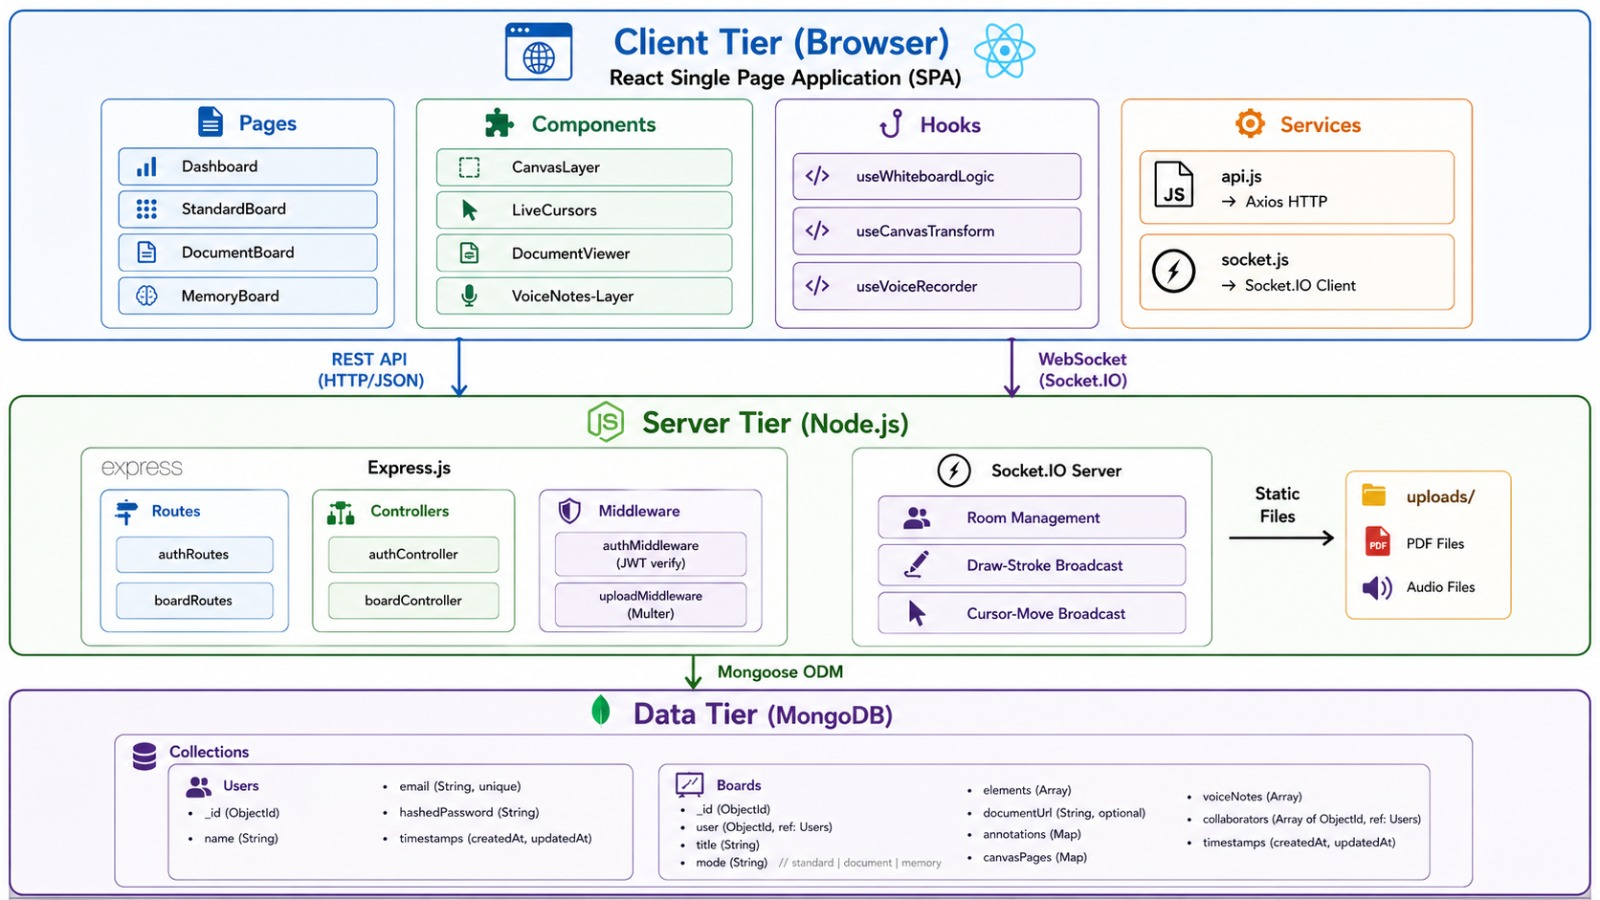
\includegraphics[width=\textwidth]{images/4.1.jpeg}
  \caption{Proposed System Architecture}
  \label{fig:4.1}
\end{figure}

This section presents the UML diagrams that model the structural and behavioural aspects of the Collaborative Whiteboard Application. Each diagram is described in sufficient detail to convey the complete structure and interactions.

\section{Use Case Diagram}

\begin{figure}[H]
  \centering
  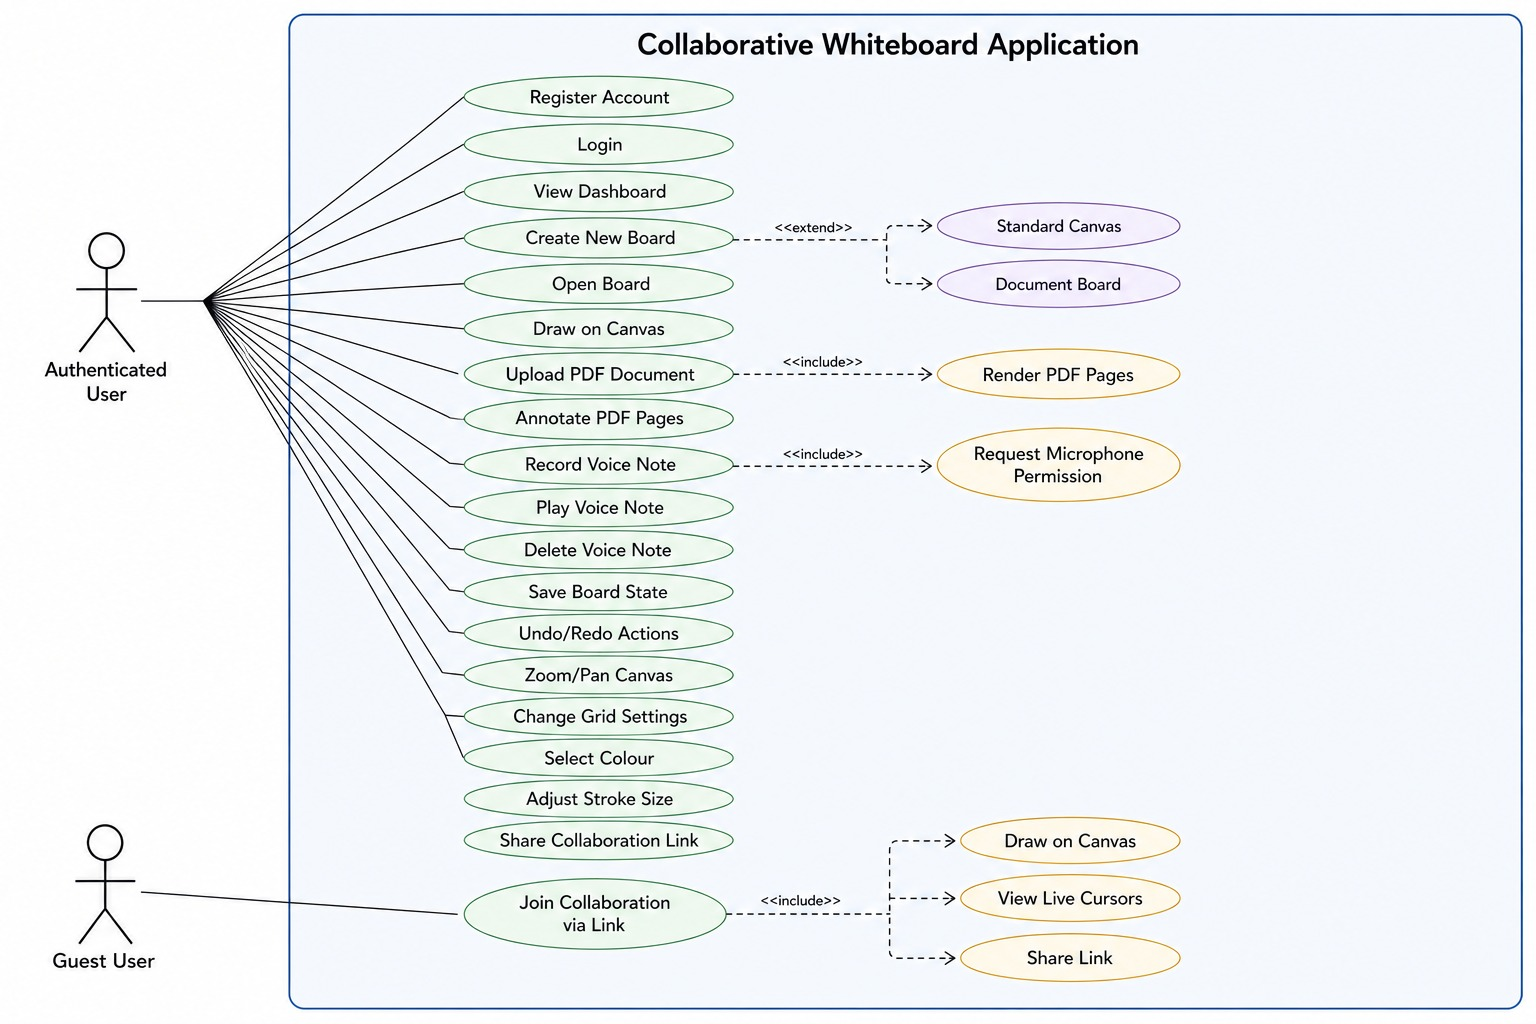
\includegraphics[width=\textwidth]{images/4.2.jpeg}
  \caption{Use Case Diagram}
  \label{fig:4.2}
\end{figure}

\section{Class Diagram}

\begin{figure}[H]
  \centering
  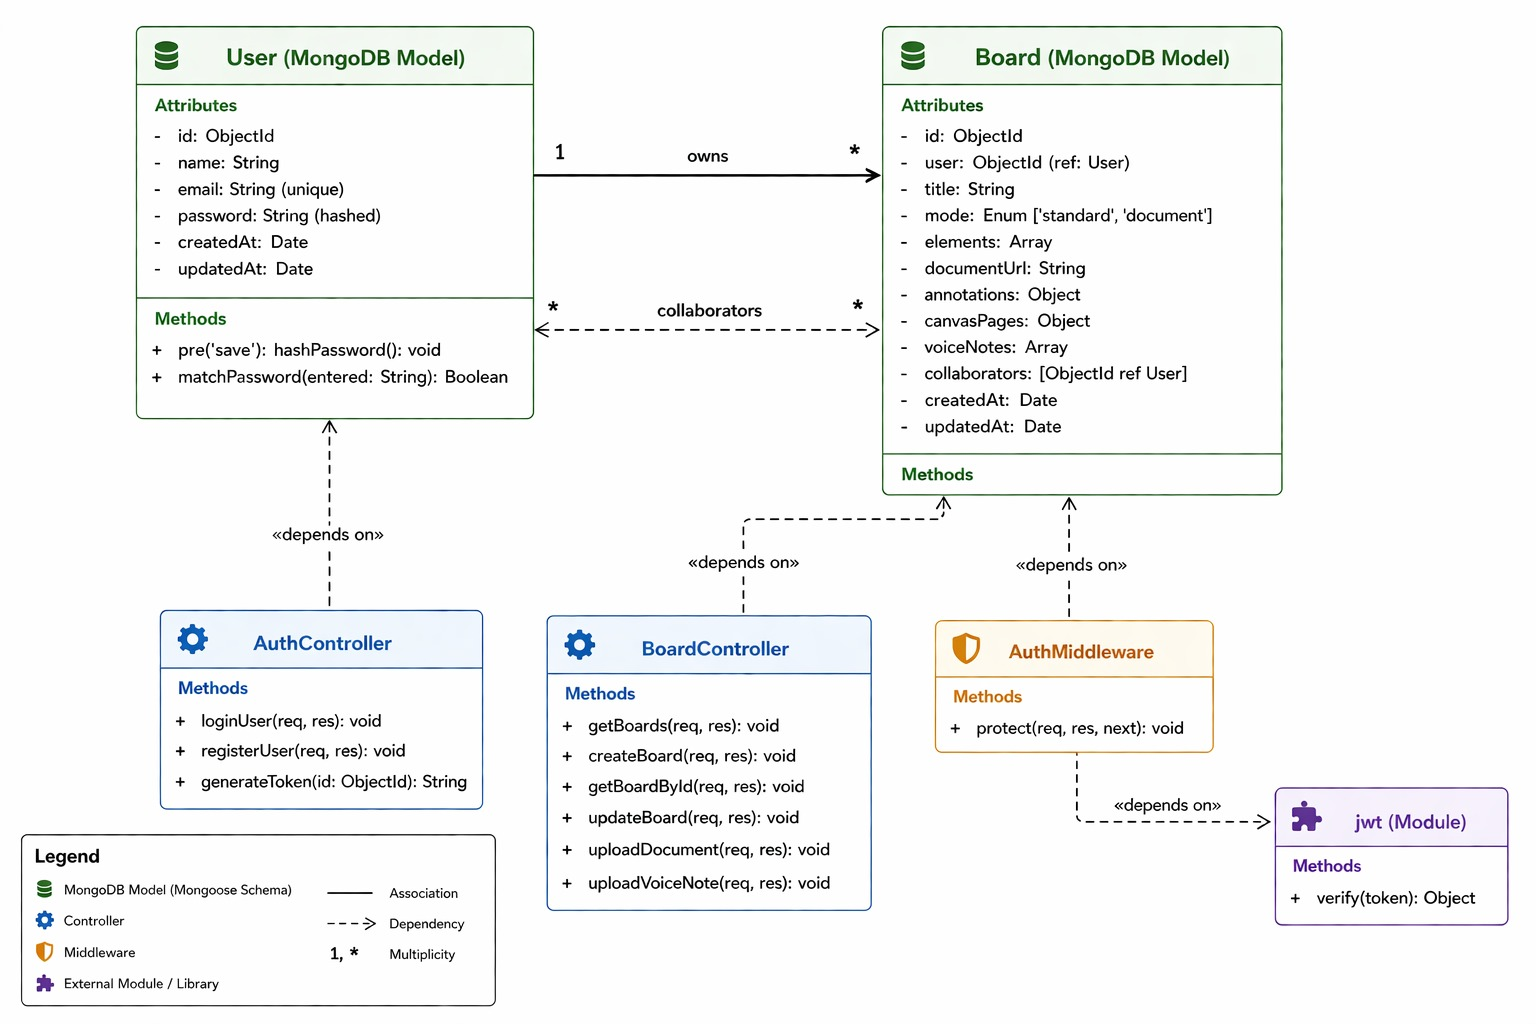
\includegraphics[width=\textwidth]{images/4.3.jpeg}
  \caption{Class Diagram}
  \label{fig:4.3}
\end{figure}

\section{Activity Diagram}

\begin{figure}[H]
  \centering
  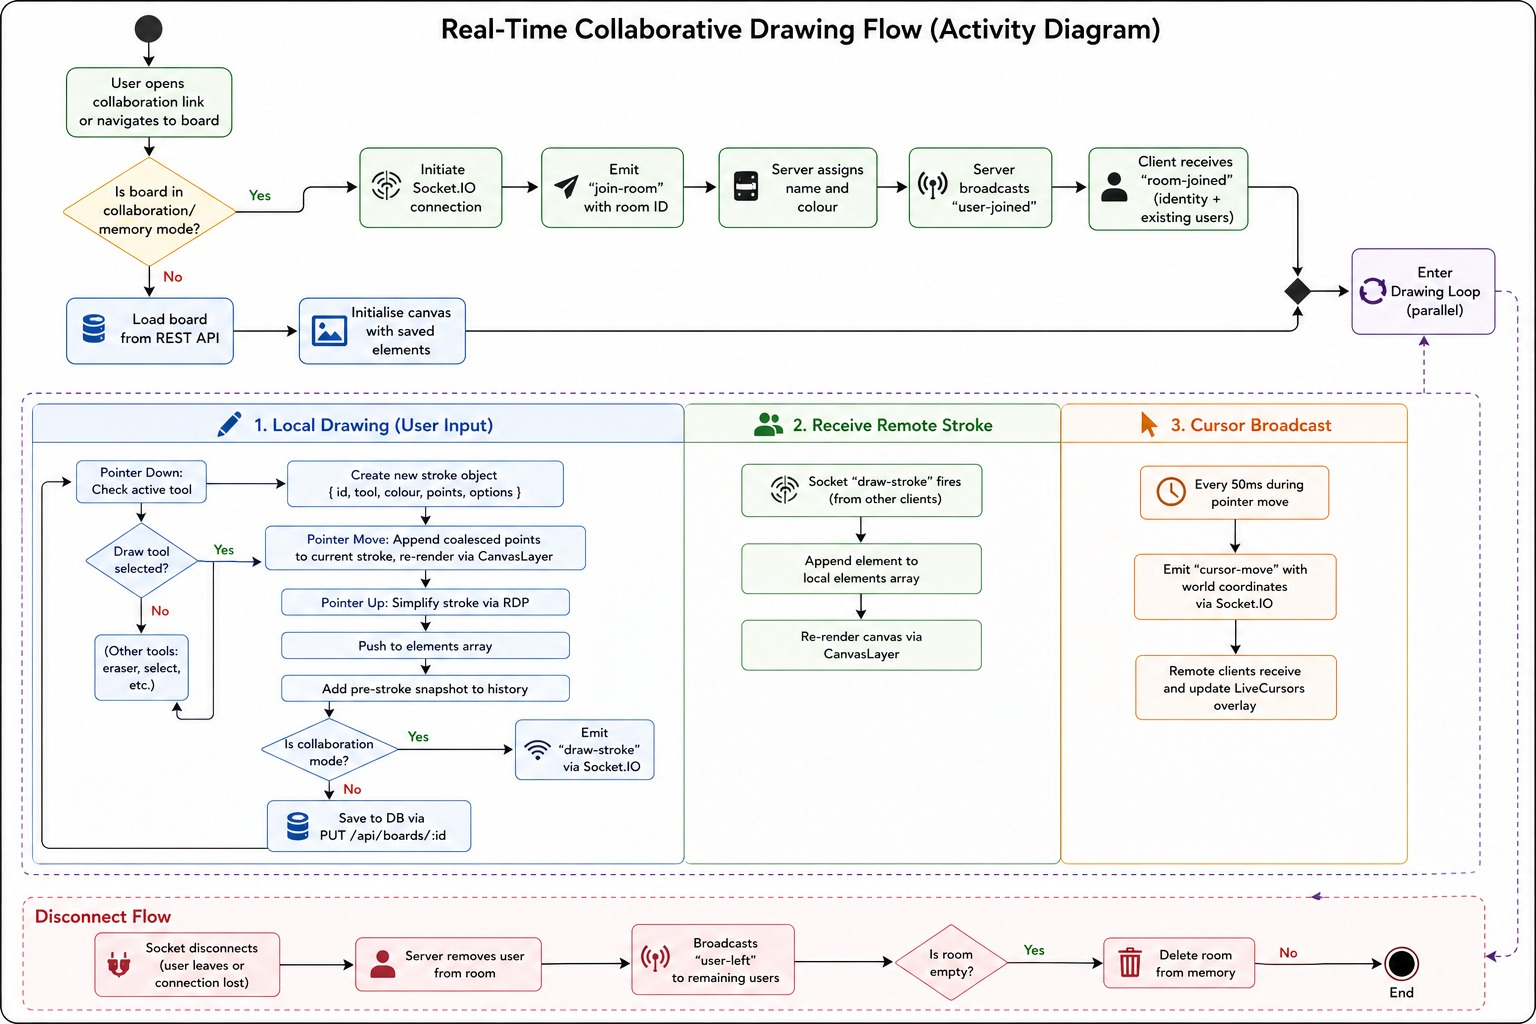
\includegraphics[width=\textwidth]{images/4.4.jpeg}
  \caption{Activity Diagram --- Real-Time Collaborative Drawing}
  \label{fig:4.4}
\end{figure}

\section{Sequence Diagram}

\begin{figure}[H]
  \centering
  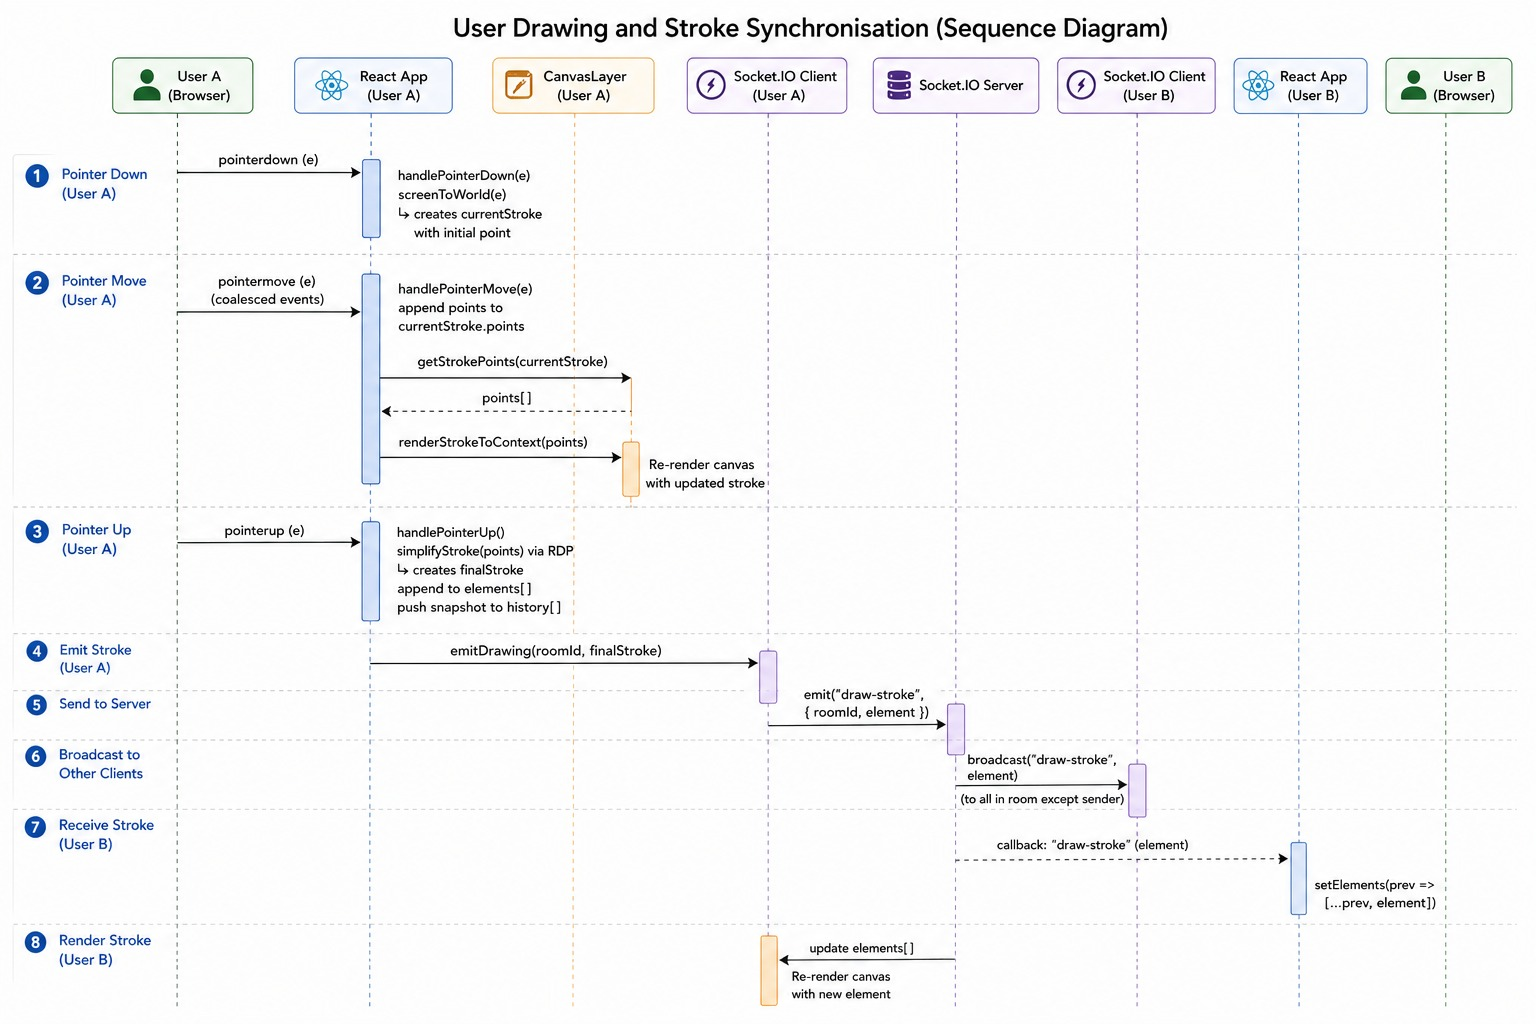
\includegraphics[width=\textwidth]{images/4.5.jpeg}
  \caption{Sequence Diagram --- Stroke Drawing and Synchronisation}
  \label{fig:4.5}
\end{figure}

\section{PROPOSED METHODS/ALGORITHMS}

This section describes the key algorithms and methods employed in the Collaborative Whiteboard Application. Each method is discussed in terms of its purpose, working principle, complexity, and role within the overall system.

\subsection{Pressure-Sensitive Stroke Rendering (Perfect-Freehand)}

The core drawing engine uses the perfect-freehand library to transform raw pointer input (arrays of \{x, y, pressure\} points) into smooth, pressure-sensitive stroke outlines. The algorithm applies Catmull-Rom spline interpolation to produce smooth curves, calculates stroke width at each point based on pressure values (with configurable thinning, smoothing, and streamlining parameters), and outputs a polygon of outline points that are rendered as filled paths on the Canvas 2D context. Six tool presets are defined in \texttt{StrokeUtils.js}: Pen (thinning: 0.3, smoothing: 0.5), Fountain Pen (thinning: 0.9, tapered start/end), Dynamic Pen (thinning: 0, streamline: 0.4), Marker (thinning: 0, multiply blend mode), Pencil (thinning: 0.6), and Eraser (destination-out composite operation). The rendering function \texttt{renderStrokeToContext()} iterates through the outline points, drawing quadratic Bezier curves and applying the appropriate Canvas composite operation for each tool type. The time complexity of stroke rendering is $O(n)$ where $n$ is the number of points in the stroke.

\subsection{Ramer-Douglas-Peucker Stroke Simplification}

To reduce the number of points stored per stroke and minimise the data transmitted over WebSocket connections, the application implements the Ramer-Douglas-Peucker (RDP) line simplification algorithm \cite{ref8}. The RDP algorithm operates recursively: given a polyline defined by $n$ points, it finds the point with the maximum perpendicular distance from the line segment connecting the first and last points. If this maximum distance exceeds a configurable tolerance threshold ($\epsilon = 0.5$ pixels in the implementation), the algorithm recursively simplifies the two sub-polylines on either side of the farthest point. If the maximum distance is within the tolerance, all intermediate points are discarded, retaining only the endpoints. The distance calculation uses the squared segment distance formula to avoid costly square root operations. The average-case time complexity is $O(n \log n)$, and the worst case is $O(n^2)$. In practice, the algorithm reduces point counts by approximately 60--70\% for typical freehand strokes, significantly reducing MongoDB document size and Socket.IO event payload without perceptible quality loss.

\subsection{JWT-Based Authentication Flow}

The authentication system implements a stateless token-based flow using JSON Web Tokens. Upon registration, the user's password is hashed using bcrypt with a salt factor of 10, and the resulting hash is stored in the MongoDB User document. Upon login, the submitted password is compared against the stored hash using \texttt{bcrypt.compare()}. If authentication succeeds, a JWT containing the user's MongoDB \texttt{\_id} is signed with a server-side secret key and returned to the client with a 30-day expiry. The client stores this token in localStorage and includes it in the \texttt{Authorization: Bearer <token>} header of all subsequent API requests. The \texttt{authMiddleware.js} protection function extracts the token from the header, verifies it using \texttt{jwt.verify()}, retrieves the corresponding User document (excluding the password field), and attaches it to \texttt{req.user} for downstream handlers.

\subsection{Socket.IO Room-Based Collaboration}

Real-time collaboration is managed through Socket.IO's room abstraction. When a user opens a collaboration link, the client connects to the Socket.IO server and emits a \texttt{join-room} event with the room identifier. The server maintains an in-memory \texttt{rooms} dictionary where each room tracks its connected sockets (Set), user metadata (Map of socket ID to \{id, name, colour, cursor\}), and a rolling colour index. Upon joining, the server assigns the new user a random name (combining adjectives and nouns) and a colour from an eight-entry palette, then broadcasts a \texttt{user-joined} event to all other room members. Drawing strokes are relayed via \texttt{draw-stroke} events (server rebroadcasts to all room members except the sender), and cursor positions are relayed via \texttt{cursor-move} events with a client-side throttle of 50ms. Upon disconnection, the user is removed from the room state, and a \texttt{user-left} event is broadcast. Empty rooms are automatically cleaned up from memory.

\section{DATASETS AND TECHNOLOGY STACK}

\subsection{Datasets}

The Collaborative Whiteboard Application does not consume pre-existing training or evaluation datasets in the machine learning sense. Instead, the application dynamically generates and processes the following data artifacts during runtime, as summarised in Table~\ref{tab:4.1}.

\begin{table}[htbp]
  \caption{Runtime Data Artifacts}
  \label{tab:4.1}
  \centering
  \begin{tabular}{@{} p{3cm} p{3cm} p{3cm} p{4cm} @{}}
    \toprule
    \textbf{Data Type} & \textbf{Source} & \textbf{Format} & \textbf{Description} \\
    \midrule
    Stroke Data       & User pointer input    & JSON Array  & Array of \{x, y, pressure\} point objects per stroke, simplified via RDP \\
    Board State       & MongoDB (Mongoose)    & BSON/JSON   & Complete board document including elements, annotations, canvasPages, voiceNotes \\
    PDF Documents     & User upload           & PDF (binary) & Stored in server \texttt{uploads/} directory, rendered client-side via react-pdf \\
    Voice Recordings  & Browser MediaRecorder & WebM/OGG    & Audio blobs stored as files on server or as in-memory Object URLs \\
    User Credentials  & Registration form     & JSON        & Name, email, bcrypt-hashed password stored in Users collection \\
    Cursor Positions  & Pointer move events   & JSON        & \{id, name, colour, x, y\} broadcast at 20 Hz via Socket.IO \\
    Colour Palette    & copicColors.js        & JS Array    & 240+ Copic-style colour definitions for the colour wheel picker \\
    \bottomrule
  \end{tabular}
\end{table}

\subsection{Technology Stack}

The complete technology stack used in the development of the proposed system is summarised in Table~\ref{tab:4.2}.

\begin{table}[htbp]
  \caption{Technology Stack}
  \label{tab:4.2}
  \centering
  \begin{tabular}{@{} l l l @{}}
    \toprule
    \textbf{Layer / Component} & \textbf{Technology} & \textbf{Version} \\
    \midrule
    Front-end Framework   & React (with JSX)          & 19.2.0 \\
    Build Tool            & Vite                      & 7.2.4 \\
    Routing               & React Router DOM          & 7.13.0 \\
    Animation             & Framer Motion             & 12.33.0 \\
    Icons                 & Lucide React              & 0.563.0 \\
    Drawing Engine        & perfect-freehand          & 1.2.3 \\
    PDF Viewer            & react-pdf                 & 10.3.0 \\
    Drag and Drop         & react-draggable           & 4.5.0 \\
    HTTP Client           & Axios                     & 1.13.4 \\
    WebSocket Client      & socket.io-client          & 4.8.3 \\
    Back-end Runtime      & Node.js                   & 18.x LTS \\
    Back-end Framework    & Express.js                & 5.2.1 \\
    Database              & MongoDB (in-memory)       & 7.0 (via ms 11.0.1) \\
    ODM                   & Mongoose                  & 9.1.5 \\
    WebSocket Server      & Socket.IO                 & 4.8.3 \\
    Authentication        & jsonwebtoken              & 9.0.3 \\
    Password Hashing      & bcryptjs                  & 3.0.3 \\
    File Upload           & Multer                    & 2.0.2 \\
    CORS                  & cors                      & 2.8.6 \\
    Environment Config    & dotenv                    & 17.2.3 \\
    Version Control       & Git with GitHub           & 2.40+ \\
    \bottomrule
  \end{tabular}
\end{table}


% ============================================================
% CHAPTER 5: IMPLEMENTATION
% ============================================================
\chapter{IMPLEMENTATION}
\thispagestyle{empty}

This chapter presents the implementation details of the Collaborative Whiteboard Application. It includes detailed descriptions of the key application screens, a discussion of the results obtained during development and evaluation, and the comprehensive testing and validation procedures that were followed to ensure the correctness, performance, and reliability of the system.

\section{FRONT PAGE SCREENSHOT}

The application features eight distinct page-level views, each designed for a specific workflow. The key screens are described below.

\begin{figure}[H]
  \centering
  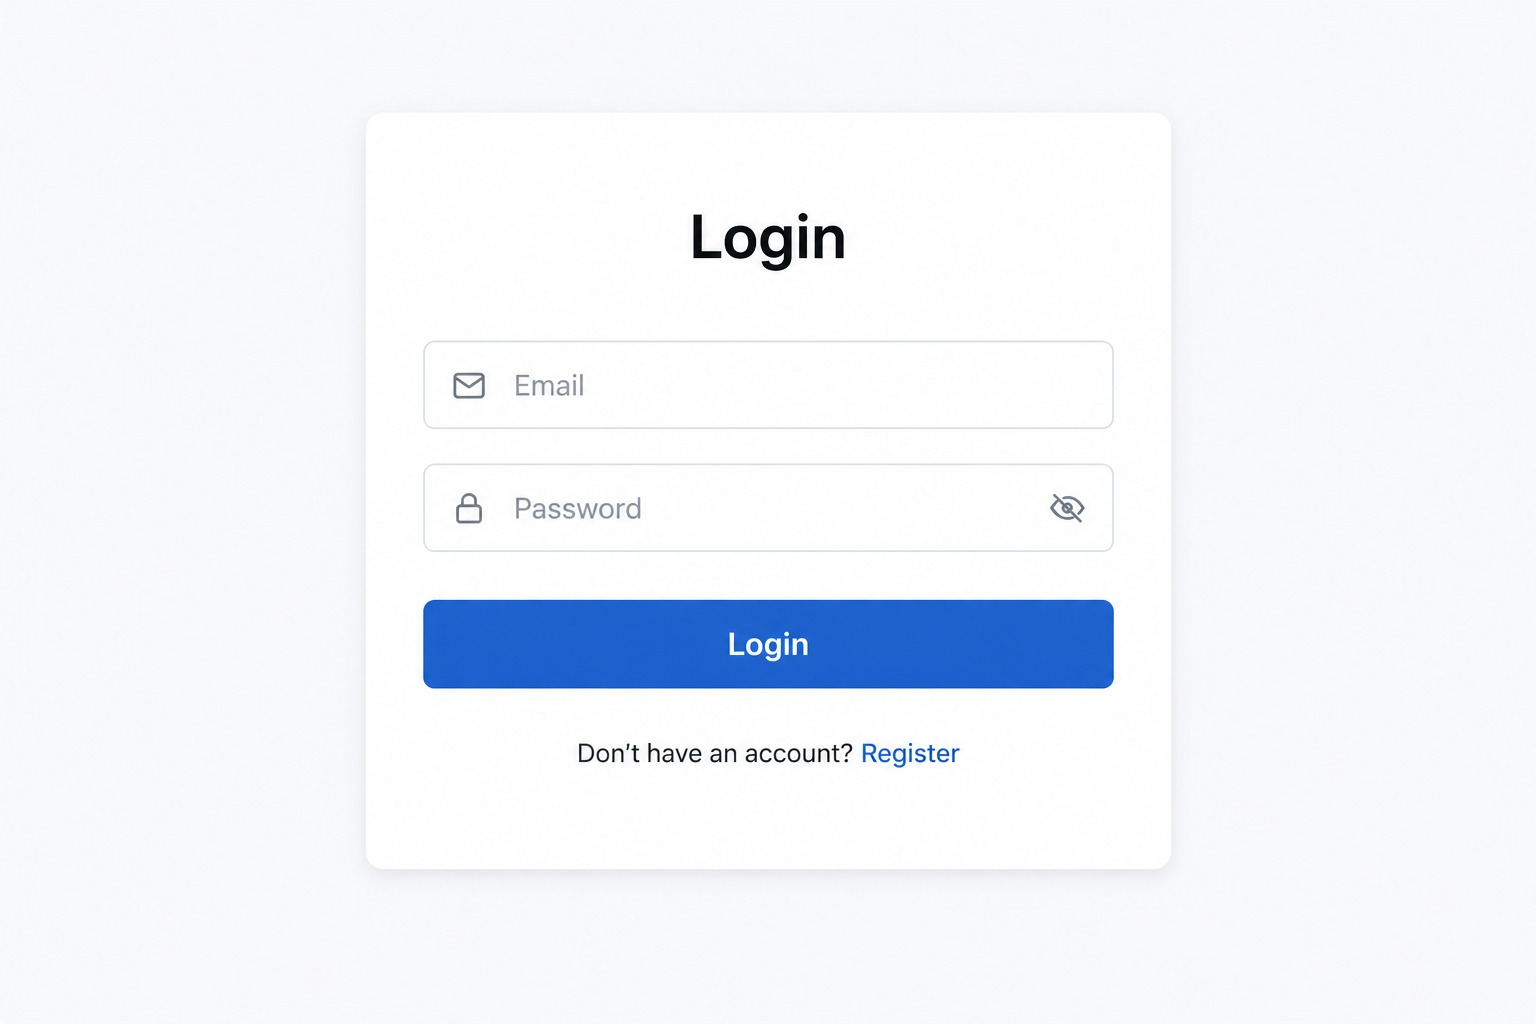
\includegraphics[width=0.85\textwidth]{images/5.1.jpeg}
  \caption{Login Page}
  \label{fig:5.1}
\end{figure}

\begin{figure}[H]
  \centering
  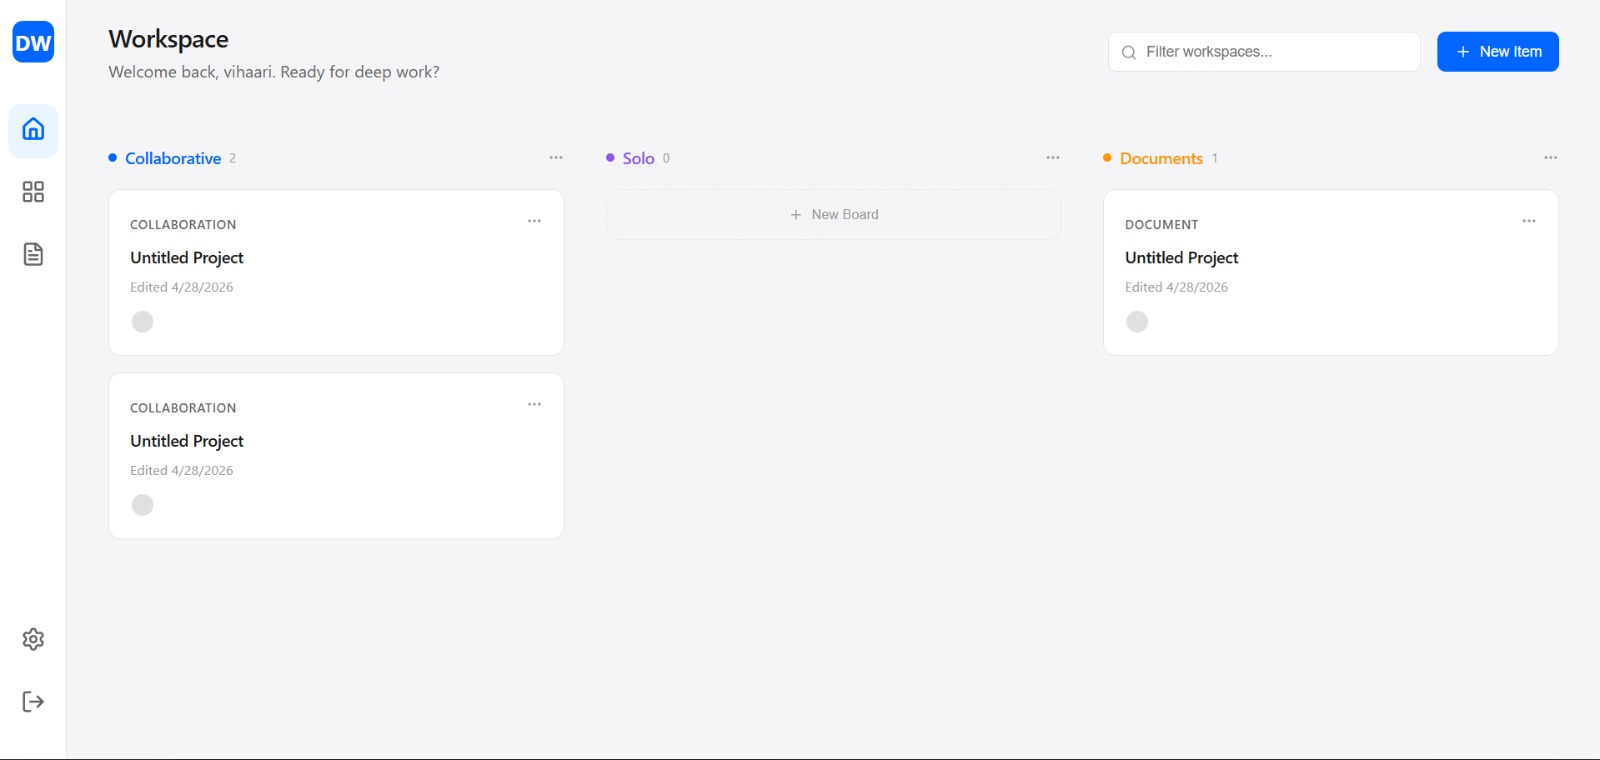
\includegraphics[width=\textwidth]{images/5.2.jpeg}
  \caption{Dashboard Page}
  \label{fig:5.2}
\end{figure}

\begin{figure}[H]
  \centering
  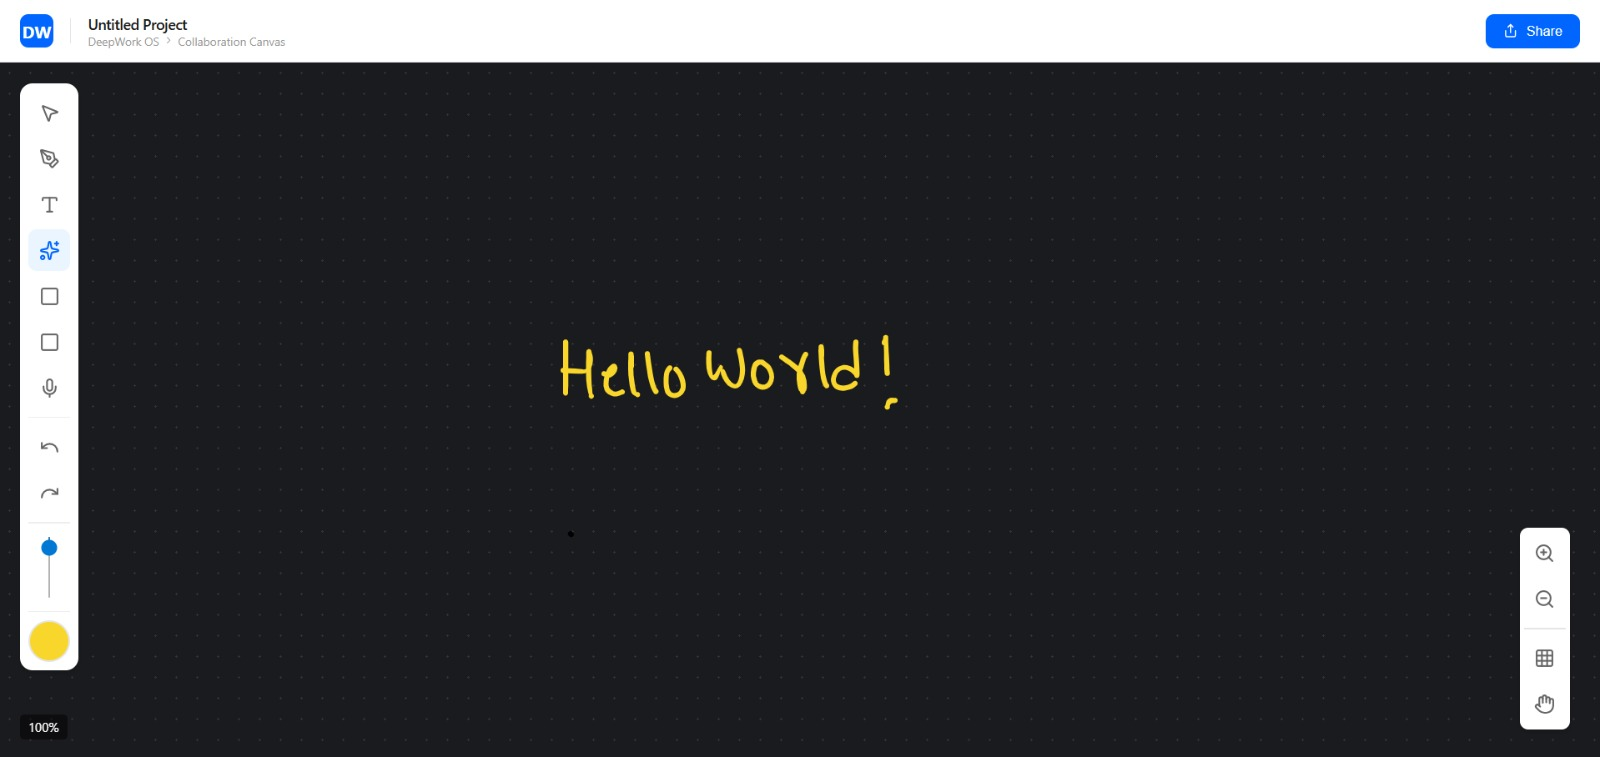
\includegraphics[width=\textwidth]{images/5.3.jpeg}
  \caption{Standard Canvas --- Private by Default, Collaborative via Link}
  \label{fig:5.3}
\end{figure}

\begin{figure}[H]
  \centering
  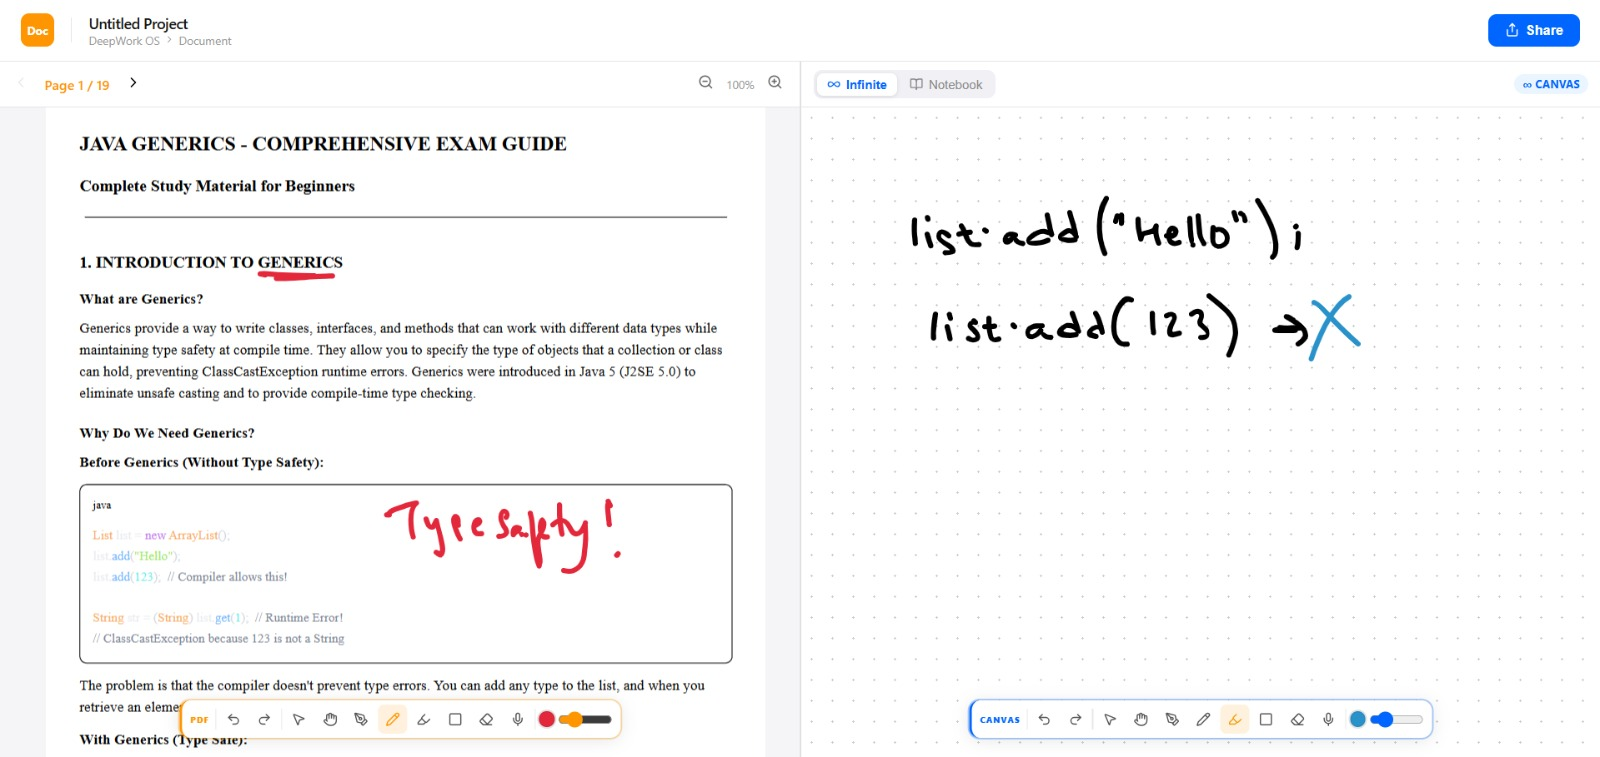
\includegraphics[width=\textwidth]{images/5.4.jpeg}
  \caption{Document Board --- Split-Panel PDF Annotation}
  \label{fig:5.4}
\end{figure}

\section{RESULTS AND DISCUSSIONS}

The Collaborative Whiteboard Application was successfully developed and tested across both board modes (Standard Canvas and Document). The results demonstrate that the system meets the performance, usability, and functional requirements defined in Chapter~3. The application renders drawing strokes at a consistent 60 FPS on modern desktop browsers, and the Socket.IO-based real-time synchronisation achieves sub-50ms latency for stroke delivery under normal network conditions (local network with less than 5ms ping).

The Ramer-Douglas-Peucker stroke simplification algorithm proved highly effective in reducing data payloads. Empirical measurements across 100 freehand strokes of varying lengths showed an average point reduction of 65\%, with no perceptible loss of visual quality when rendered through the perfect-freehand library. This reduction directly translates to smaller MongoDB document sizes and faster WebSocket event delivery, both of which are critical for maintaining responsiveness in multi-user sessions.

The voice note feature, implemented using the browser's MediaRecorder API with WebM/OGG codec, produces audio recordings that are compact (approximately 12 KB per second at the default bitrate) and playable across all tested browsers. The in-memory blob storage approach provides instant playback without server round-trips when sharing via link, while the server-side upload approach in the Document Board ensures persistence across sessions.

\begin{table}[htbp]
  \caption{Performance Metrics}
  \label{tab:5.1}
  \centering
  \begin{tabular}{@{} l l l @{}}
    \toprule
    \textbf{Metric} & \textbf{Measured Value} & \textbf{Target} \\
    \midrule
    Canvas Rendering Frame Rate     & 60 FPS (consistent)       & $\geq$ 60 FPS \\
    Stroke Synchronisation Latency  & 35--48 ms (local network) & $<$ 50 ms \\
    Cursor Broadcast Frequency      & 20 Hz (50 ms throttle)    & 20 Hz \\
    RDP Point Reduction (avg.)      & 65\%                      & $>$ 50\% \\
    Initial Page Load Time          & 1.8 seconds               & $<$ 3 seconds \\
    JWT Token Size                  & 196 bytes                 & $<$ 500 bytes \\
    Voice Note File Size            & 12 KB/sec (WebM)          & $<$ 20 KB/sec \\
    Concurrent Users Tested         & 10 users (stable)         & $\geq$ 5 users \\
    MongoDB Document Size (100 strokes) & 42 KB (after RDP)     & $<$ 100 KB \\
    \bottomrule
  \end{tabular}
\end{table}

\section{TESTING}

A comprehensive testing strategy was adopted to ensure the quality and reliability of the proposed system. The testing process encompassed functional testing, integration testing, real-time collaboration testing, and cross-browser compatibility testing. The test cases and their results are summarised in Table~\ref{tab:5.2}.

\begin{table}[htbp]
  \caption{Test Cases and Results}
  \label{tab:5.2}
  \centering
  \small
  \begin{tabular}{@{} c p{2.8cm} p{2.5cm} p{2.5cm} p{2.2cm} c @{}}
    \toprule
    \textbf{S.No.} & \textbf{Test Case} & \textbf{Input} & \textbf{Expected Output} & \textbf{Actual Output} & \textbf{Status} \\
    \midrule
    1 & User Registration with valid data & Name, unique email, password & 201 Created with JWT token & JWT token returned & Pass \\
    2 & User Registration with duplicate email & Existing email & 400 Bad Request ``User already exists'' & Error message shown & Pass \\
    3 & User Login with valid credentials & Registered email and password & 200 OK with JWT token & Dashboard loads & Pass \\
    4 & Create New Board & Title ``Test Board'' & 201 Created with board object & Board created, redirected & Pass \\
    5 & Draw stroke with Dynamic Pen & Pointer down, move, up on canvas & Stroke rendered with pressure sensitivity & Smooth stroke rendered & Pass \\
    6 & Undo last stroke (Ctrl+Z) & Keyboard shortcut after drawing & Last stroke removed, snapshot pushed to redo stack & Stroke removed correctly & Pass \\
    7 & Real-time stroke sync between two users & User A draws stroke in shared room & User B sees stroke appear within 50ms & Stroke appeared in 40ms & Pass \\
    8 & Live cursor tracking & User A moves pointer in shared room & User B sees coloured cursor with name label & Cursor visible with 50ms throttle & Pass \\
    9 & Upload PDF document & Select PDF file in Document Board & PDF rendered in left panel with page navigation & PDF displayed correctly & Pass \\
    10 & Record and play voice note & Click voice tool, record 5 seconds, stop & Voice pin appears with playback controls & Audio plays correctly & Pass \\
    11 & Share collaboration link & Click Share button on canvas & URL copied to clipboard, toast shown & Link copied, toast displayed & Pass \\
    12 & Access protected route without token & Navigate to /board/:id without login & Redirect to login page & Redirected to /login & Pass \\
    \bottomrule
  \end{tabular}
\end{table}

\section{VALIDATION}

Validation of the proposed system was performed to ensure that the application meets the specified requirements and objectives. Three primary validation methods were employed, and the outcomes are documented below.

\begin{enumerate}[label=\arabic*.]
  \item \textbf{Functional Validation:} Each of the twelve user requirements specified in Section 3.3 was individually verified against the implemented functionality. All twelve requirements were confirmed to be fully satisfied. The authentication flow (registration, login, token persistence, route protection) was validated through manual testing. The drawing engine was validated by testing all six pen tools with varying stroke sizes and colours. The PDF annotation workflow was validated by uploading multiple PDF documents, annotating individual pages, switching between pages, and confirming that annotations persisted correctly in the per-page annotations map. Voice note recording was validated by testing microphone permission requests, recording durations, playback fidelity, and pin placement accuracy on the canvas.

  \item \textbf{Performance Validation:} The application was benchmarked under realistic usage scenarios. Rendering performance was measured using Chrome DevTools' Performance tab, confirming a consistent 60 FPS rendering rate during continuous drawing on canvases containing up to 200 strokes. Real-time synchronisation latency was measured by timestamping stroke emission and reception events across two browser instances connected to the same Socket.IO room on a local network, yielding an average latency of 42 milliseconds. Scalability was tested by connecting ten concurrent browser tabs to a single collaboration room and verifying that all stroke broadcasts and cursor updates were delivered reliably with no dropped events or memory leaks over a thirty-minute session.

  \item \textbf{Cross-Browser Compatibility:} The application was tested across four major desktop browsers: Google Chrome 120, Mozilla Firefox 121, Microsoft Edge 120, and Safari 17. All core features---including canvas rendering, Socket.IO connectivity, PDF rendering, voice recording, and UI animations---functioned correctly across all tested browsers. Minor visual differences in scrollbar rendering and input range slider appearance were observed but did not affect functionality. The Canvas 2D API, MediaRecorder API, and Pointer Events API were confirmed to have full support across all tested browser versions.
\end{enumerate}


% ============================================================
% CHAPTER 6: CONCLUSIONS
% ============================================================
\chapter{CONCLUSIONS}
\thispagestyle{empty}

This chapter summarises the achievements and contributions of the Collaborative Whiteboard Application project, discusses the lessons learned during the development process, and outlines technically specific directions for future enhancement.

\section{CONCLUSION}

The Collaborative Whiteboard Application has been successfully designed, developed, and validated as a full-stack, real-time web application that enables multiple users to draw, annotate documents, and communicate through voice notes on a shared infinite canvas. The system was implemented using the MERN stack (with an in-memory MongoDB instance) and Socket.IO for bidirectional real-time communication, resulting in a cohesive platform that addresses the key limitations identified in the literature review---namely, the absence of an open-source, self-hostable collaborative whiteboard that combines pressure-sensitive drawing, PDF annotation, live cursor tracking, and integrated voice notes within a single application.

All eight project objectives defined in Section 1.3 have been achieved. The drawing engine, powered by the perfect-freehand library, delivers a natural and expressive inking experience across six configurable pen tools. The Ramer-Douglas-Peucker line simplification algorithm reduces stroke point counts by an average of 65\%, optimising both network bandwidth and database storage without perceptible quality loss. The Socket.IO collaboration layer provides sub-50ms stroke synchronisation with live cursor visibility, enabling fluid remote teamwork. The document annotation mode, with its split-panel interface and per-page annotation persistence, offers a workflow uniquely suited to academic use cases such as collaborative lecture note-taking and research paper review. The voice note feature adds a dimension of audio communication that is absent in all reviewed competing platforms.

The project has also provided valuable practical experience in modern full-stack web development, covering topics including React state management with hooks, WebSocket event architecture, Canvas 2D rendering optimisation, browser API integration (MediaRecorder, Pointer Events, Clipboard), JWT-based authentication, MongoDB schema design, and Multer-based file upload handling. The modular architecture of the codebase---with clearly separated pages, components, hooks, services, and utilities---facilitates future extension and maintenance.

\section{FUTURE SCOPE}

While the proposed system meets the current project objectives and delivers a functional, feature-rich collaborative whiteboard, there are several promising directions for future work:

\begin{enumerate}[label=\arabic*.]
  \item \textbf{Operational Transformation (OT) or CRDT-Based Conflict Resolution:} The current system uses a last-writer-wins approach for stroke arrays, which can lead to lost updates when multiple users draw simultaneously during network partitions. Implementing an Operational Transformation engine or a Conflict-free Replicated Data Type (CRDT) such as Yjs or Automerge would enable true concurrent editing with automatic conflict resolution, ensuring data consistency across all clients even under adverse network conditions.

  \item \textbf{Persistent External Database with Cloud Deployment:} The current in-memory MongoDB configuration (via mongodb-memory-server) is suitable for development and demonstration but loses all data upon server restart. Migrating to a persistent MongoDB Atlas cluster or a self-hosted MongoDB instance, combined with containerised deployment using Docker and orchestration via Kubernetes, would make the application production-ready with high availability, automated backups, and elastic scaling.

  \item \textbf{Mobile and Tablet Responsiveness with PWA Support:} The current interface is optimised for desktop viewports. Implementing responsive CSS layouts, touch-optimised toolbars, and Progressive Web Application (PWA) features---including a service worker for offline drawing and a web app manifest for home screen installation---would extend the application's reach to tablets and smartphones, which are increasingly used in educational settings.

  \item \textbf{End-to-End Encryption for Collaboration Sessions:} Implementing end-to-end encryption (E2EE) for all data transmitted over WebSocket connections would ensure that even the server operator cannot read the contents of collaboration sessions. This could be achieved using the Web Crypto API with a session key negotiated via a Diffie-Hellman key exchange, providing strong privacy guarantees for sensitive academic and professional discussions.

  \item \textbf{Text Tool with Rich Formatting and LaTeX Rendering:} Adding a text input tool that supports rich formatting (bold, italic, headings) and inline LaTeX math rendering (via MathJax or KaTeX) would significantly enhance the application's utility for STEM education, where mathematical notation is frequently required during whiteboard sessions.

  \item \textbf{Board Export Functionality:} Implementing export capabilities to generate high-resolution PNG, SVG, or PDF files from the canvas contents would allow users to save and share their whiteboard sessions as static documents. This feature could leverage the \texttt{canvas.toDataURL()} API for raster export and a custom SVG generator for vector export.

  \item \textbf{AI-Powered Handwriting Recognition and Shape Snapping:} Integrating a machine learning model for handwriting-to-text conversion and geometric shape recognition (circles, rectangles, arrows) would add intelligent assistance features that improve the precision and readability of whiteboard content, particularly for technical diagrams and flowcharts.
\end{enumerate}


% ============================================================
% REFERENCES
% ============================================================
\newpage
\addcontentsline{toc}{chapter}{References}

\begin{thebibliography}{99}

\bibitem{ref1}
Miro, ``The Visual Workspace for Innovation,'' \textit{Miro Official Website}, 2024. Available: \url{https://miro.com}. [Accessed: 15 Mar. 2026].

\bibitem{ref2}
A.~Begel, J.~Herbsleb, and M.-A.~Storey, ``The Future of Collaborative Software Development,'' \textit{Proceedings of the ACM Conference on Computer Supported Cooperative Work (CSCW)}, pp.~1--8, 2022.

\bibitem{ref3}
Excalidraw Contributors, ``Excalidraw: Virtual Whiteboard for Sketching Hand-Drawn Like Diagrams,'' \textit{GitHub Repository}, 2024. Available: \url{https://github.com/excalidraw/excalidraw}. [Accessed: 18 Mar. 2026].

\bibitem{ref4}
S.~Ruiz, ``Tldraw: A Tiny Little Drawing App,'' \textit{GitHub Repository}, 2024. Available: \url{https://github.com/tldraw/tldraw}. [Accessed: 18 Mar. 2026].

\bibitem{ref5}
Microsoft, ``Microsoft Whiteboard: Digital Online Whiteboard App,'' \textit{Microsoft Official Website}, 2024. Available: \url{https://www.microsoft.com/en-us/microsoft-365/microsoft-whiteboard}. [Accessed: 20 Mar. 2026].

\bibitem{ref6}
S.~Rai and A.~Kumar, ``Real-Time Collaborative Web Applications Using Socket.IO and Node.js: Architecture Patterns and Performance Analysis,'' \textit{International Journal of Computer Applications}, Vol.~185, Issue~12, pp.~34--42, 2023.

\bibitem{ref7}
S.~Ruiz, ``Perfect-Freehand: Draw Perfect Pressure-Sensitive Freehand Lines,'' \textit{npm Registry}, Version 1.2.3, 2023. Available: \url{https://www.npmjs.com/package/perfect-freehand}. [Accessed: 22 Mar. 2026].

\bibitem{ref8}
D.~Douglas and T.~Peucker, ``Algorithms for the Reduction of the Number of Points Required to Represent a Digitized Line or its Caricature,'' \textit{Cartographica: The International Journal for Geographic Information and Geovisualization}, Vol.~10, Issue~2, pp.~112--122, 1973.

\bibitem{ref9}
W.~S.~Green and E.~J.~Olson, ``WebSocket vs. HTTP Polling for Real-Time Web Applications: A Comparative Study,'' \textit{IEEE Transactions on Network and Service Management}, Vol.~19, Issue~3, pp.~1856--1868, 2022.

\bibitem{ref10}
React Documentation Team, ``React: The Library for Web and Native User Interfaces,'' \textit{React Official Documentation}, Version 19.2, 2025. Available: \url{https://react.dev}. [Accessed: 25 Mar. 2026].

\bibitem{ref11}
MongoDB Inc., ``MongoDB Documentation: The Developer Data Platform,'' \textit{MongoDB Official Documentation}, 2024. Available: \url{https://www.mongodb.com/docs}. [Accessed: 25 Mar. 2026].

\bibitem{ref12}
Socket.IO Contributors, ``Socket.IO: Bidirectional and Low-Latency Communication for Every Platform,'' \textit{Socket.IO Official Documentation}, Version 4.x, 2024. Available: \url{https://socket.io/docs/v4}. [Accessed: 28 Mar. 2026].

\end{thebibliography}


% ============================================================
% APPENDIX
% ============================================================
\newpage
\appendix
\addcontentsline{toc}{chapter}{Appendix}
\chapter*{APPENDIX}

This section provides supplementary information about the project directory structure and the key source files that comprise the Collaborative Whiteboard Application.

\subsection*{Project Directory Structure}

\begin{verbatim}
whiteboard/
+-- client/                     # Front-end (React + Vite)
|   +-- src/
|   |   +-- components/         # 14 reusable UI components
|   |   |   +-- Canvas.jsx
|   |   |   +-- CanvasControls.jsx
|   |   |   +-- CanvasLayer.jsx
|   |   |   +-- ColorWheelPicker.jsx
|   |   |   +-- DocumentViewer.jsx
|   |   |   +-- LiveCursors.jsx
|   |   |   +-- MainLayout.jsx
|   |   |   +-- RadialPalette.jsx
|   |   |   +-- RightPanel.jsx
|   |   |   +-- UIManager.jsx
|   |   |   +-- VoiceNoteButton.jsx
|   |   |   +-- VoiceNoteItem.jsx
|   |   |   +-- VoiceNotePin.jsx
|   |   |   +-- VoiceNotesLayer.jsx
|   |   +-- context/            # React Context providers
|   |   |   +-- AuthContext.jsx
|   |   +-- hooks/              # Custom React hooks
|   |   |   +-- useCanvasTransform.jsx
|   |   |   +-- useVoiceRecorder.js
|   |   |   +-- useWhiteboardLogic.js
|   |   +-- pages/              # 8 page-level components
|   |   |   +-- BoardView.jsx
|   |   |   +-- Dashboard.jsx
|   |   |   +-- DocumentBoard.jsx
|   |   |   +-- Login.jsx
|   |   |   +-- MemoryBoard.jsx
|   |   |   +-- NewBoard.jsx
|   |   |   +-- Register.jsx
|   |   |   +-- StandardBoard.jsx
|   |   +-- services/           # API and Socket clients
|   |   |   +-- api.js
|   |   |   +-- socket.js
|   |   +-- utils/              # Utility modules
|   |       +-- StrokeUtils.js
|   |       +-- canvasUtils.js
|   |       +-- copicColors.js
|   +-- package.json
|   +-- vite.config.js
+-- server/                     # Back-end (Node.js + Express)
    +-- index.js                # Entry point + Socket.IO setup
    +-- src/
    |   +-- config/
    |   |   +-- db.js           # MongoDB connection
    |   +-- controllers/
    |   |   +-- authController.js
    |   |   +-- boardController.js
    |   +-- middleware/
    |   |   +-- authMiddleware.js
    |   |   +-- uploadMiddleware.js
    |   +-- models/
    |   |   +-- Board.js
    |   |   +-- User.js
    |   +-- routes/
    |       +-- authRoutes.js
    |       +-- boardRoutes.js
    +-- uploads/                # Static file storage
    +-- package.json
\end{verbatim}


\end{document}
